\section{Globale Struktur von CR-Graphen}
\label{sec/struktur_global}

%\begin{itemize}
%	\item Erklärung der globalen Struktur zugänglicher Graphen (C,D,E,F,G,H)
%	\item Ansonten wie Kapitel \ref{sec/struktur_lokal}
%\end{itemize}

Zusätzlich zur lokalen Struktur ist außerdem die globale Struktur von CR-Graphen interessant.
Der Begriff globale Struktur gibt hier an, dass der Zellgraph von $G$ bestimmte Eigenschaften erfüllen muss.

\begin{Definition}
	Der Zellgraph $C(G)$ eines Graphen $G$ wird aus dessen stabilen Partition $\mathcal{P}_G$ gebildet.
	Es handelt sich dabei um einen vollständigen Graphen, bei dem die Knoten die Zellen von $\mathcal{P}_G$ darstellen.
\end{Definition}

\subsection{Mögliche Eigenschaften von Zellgraphen}
Für das Verständnis der folgenden Eigenschaften von CR-Graphen ist es erforderlich einige Begriffe einzuführen und Eigenschaften von Zellgraphen zu erklären und zu benennen, wozu einige Definitionen folgen.
Die Knoten eines Zellgraphen, auch als Zellen bezeichnet, können dabei folgende Eigenschaften aufweisen.

\begin{Definition}
	Eine Zelle $X\in C(G)$ wird \emph{homogen} genannt, wenn der Graph $G[X]$ vollständig oder leer ist. Anderenfalls wird diese \emph{heterogen} genannt.
\end{Definition}

\begin{Definition}
	Für eine heterogene Zelle $X\in C(G)$ finden sich je nach Beschaffenheit von $G[X]$ die Bezeichnungen \emph{matching}, \emph{co-matching} oder \emph{pentagonal}.
	Eine homogene Zelle wird dagegen entweder \emph{leer} oder \emph{vollständig} genannt.
\end{Definition}

Für die Kanten eines Zellgraphen finden sich ebenfalls unterschiedliche Bezeichnungen, welche deren Beschaffenheit beschreiben.

\begin{Definition}
	Eine Kante ${X,Y}$ mit $X,Y\in C(G)$ wird \emph{isotrop} genannt, wenn der bipartite Graph $G[X,Y]$ vollständig oder leer ist. Anderenfalls wird diese \emph{anisotrop} genannt.
\end{Definition}

\begin{Definition}
	Eine anisotrope Kante ${X,Y}$ wird \emph{Konstellation} genannt, wenn $G[X,Y]$ eine disjunkte Vereinigung von Sternen ist.
	Anderenfalls wird diese \emph{Co-Konstellation} genannt.
	Bei Co-Konstellationen bildet das \glslink{bipartites_komplement}{bipartite Komplement} von $G[X,Y]$ eine disjunkte Vereinigung von Sternen.
	Eine isotrope Kante dagegen wird entweder \emph{leer} oder \emph{vollständig} genannt.
\end{Definition}

\begin{Definition}
	 Ein Pfad $X_1X_2...X_l$ in $C(G)$, bei dem jede Kante ${X_i,X_{i+1}}$ anisotrop ist, wird \emph{anisotroper Pfad} genannt. Wenn dieser Pfad einen Kreis schließt, wird er als \emph{anisotroper Zyklus} bezeichnet. Gilt für einen anisotropen Pfad $|X_1|=|X_2|=...=|X_l|$ dann wird er \emph{gleichmäßig} genannt.
\end{Definition}

\subsection{Allgemeine globale Eigenschaften von CR-Graphen}
Mit dem so gewonnenen Hintergrundwissen kann nun das folgende Lemma formuliert werden, welches globale Eigenschaften von CR-Graphen definiert.

\begin{Lemma}
	Der Zellgraph $C(G)$ eines CR-Graphen $G$ erfüllt folgende Eigenschaften:

	\begin{enumerate}[label=(\Alph*)]
		\setcounter{enumi}{2}
		\item $C(G)$ enthält keinen gleichmäßigen, anisotropen Pfad, der zwei heterogene Zellen verbindet
		\item $C(G)$ enthält keinen gleichmäßigen, anisotropen Zyklus
		\item $C(G)$ enthält weder einen anisotropen Pfad $XY_1Y_2...Y_lZ$, sodass $|X|<|Y_1|=|Y_2|=...=|Y_l|>|Z|$, noch einen anisotropen Zyklus $XY_1Y_2...Y_l$, sodass $|X|<|Y_1|=|Y_2|=...=|Y_l|$ und die Zelle $Y_l$ heterogen ist
		\item $C(G)$ enthält keinen anisotropen Pfad $XY_1Y_2...Y_l$, sodass $|X|<|Y_1|=|Y_2|=...=|Y_l|$ und die Zelle $Y_l$ heterogen ist
	\end{enumerate}
	\label{lemma:global1}
\end{Lemma}

\emph{Beweis C:} Angenommen $P$ wäre, entgegen Bedingung \emph{C}, ein gleichmäßiger, anisotroper Pfad in $C(G)$, welcher die beiden anisotropen Komponenten $X$ und $Y$ verbindet.
Da es sich um einen gleichmäßigen Pfad handelt, besitzen sämtliche Komponenten auf dem Pfad die Kardinalität $k=|X|=|Y|$.
Alle Kanten in $P$, die eine Co-Konstellation bilden, werden nun komplementiert, sodass diese eine Konstellation ergeben.
Da nun sämtliche Kanten aus $P$ eine Konstellation darstellen und die Kardinalität aller Komponenten identisch ist, können die Sterne, welche die disjunkte Vereinigung für die Konstellationen bilden nur eine einzige Form annehmen.
Diese bestehen aus einem Zentralknoten und einem Blatt, wobei diese in unterschiedlichen Komponenten liegen.
Dadurch, dass sämtliche Kanten in $P$ diese Form annehmen ergeben sich $k$ knotendisjunkte Pfade zwischen $X$ und $Y$.
Es sind also alle Knoten aus $X$ mit genau einem Knoten aus $Y$ durch einen Pfad verbunden und andersherum.
Sei $v\in X$ durch einen solchen Pfad mit seinem Gegenstück $v^*\in Y$ verbunden.
Der Pfad $P$ wird conducting genannt, wenn diese Abbildung von Knoten einen Isomorphismus von $G[X]$ auf $G[Y]$ darstellt.
Dazu müssen zwei Knoten $u,v\in X$ genau dann adjazent sein wenn ihre Gegenstücke $u^*,v^*\in Y$ adjazent sind.
Angenommen eine der beiden Komponenten ist matching und die andere ist co-matching, dann wird $P$ ebenfalls conducting genannt, wenn die Isomorphie zwischen der matching Komponente und dem Komplement der co-matching Komponente besteht.

Nachfolgend wird ein Graph $H$ erstellt werden, der nicht zu $G$ isomorph ist, welchen das Color Refinement allerdings nicht von $G$ unterscheiden kann.
Da $X$ und $Y$ heterogen sind, können die Kanten des Subgraphen $G[X]$ durch einen isomorphen aber unterschiedlichen Graphen mit der gleichen Knotenmenge $X$ ersetzt werden.
Ist $P$ in $G$ conducting, so muss $G[X]$ so ersetzt werden, dass der entstehende Pfad in $H$ nicht conducting ist, anderenfalls muss der entsprechende Pfad in $H$ conducting sein.
Ein Beispiel für ein solches Ersetzen findet sich in Abbildung \ref{fig:global_c}.\\

\begin{figure}[t]
	\centering
	\fbox{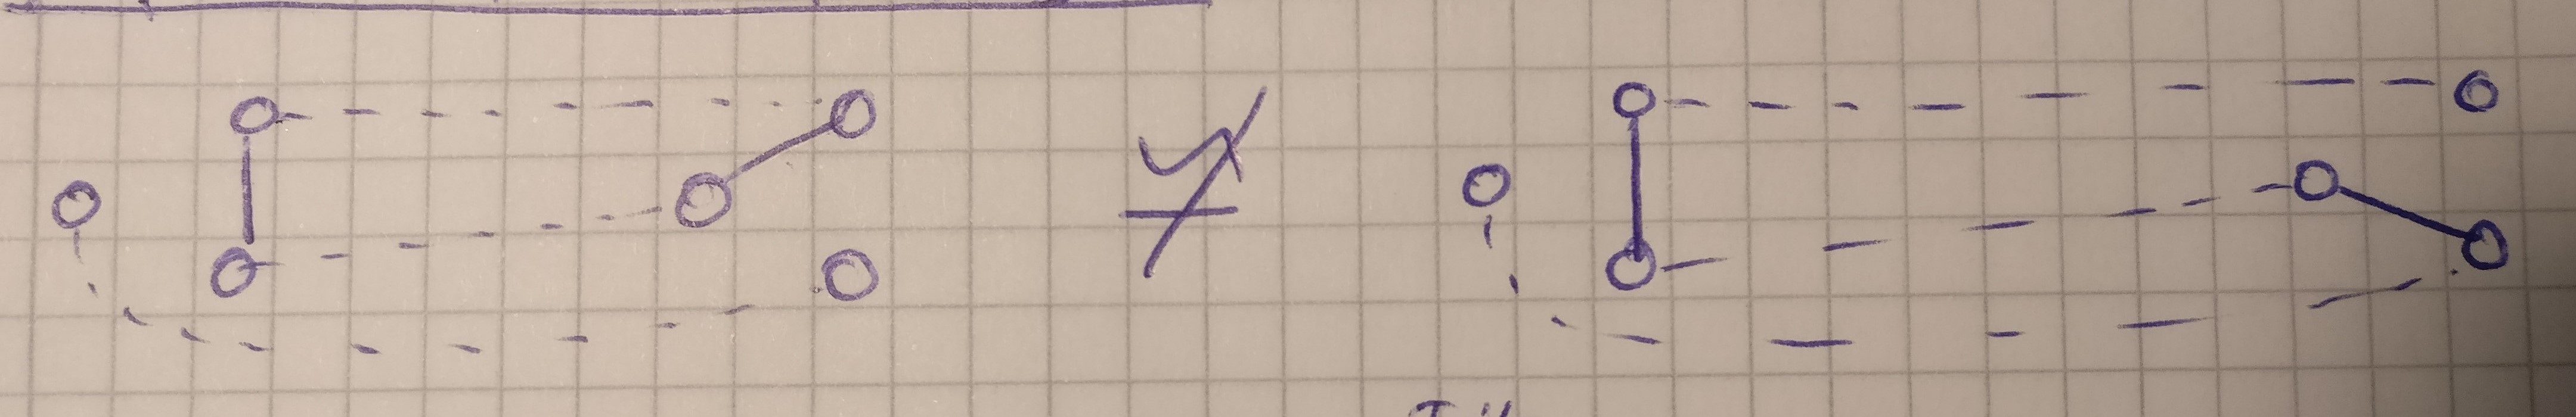
\includegraphics[width=0.75\textwidth]{./img/global_c.jpg}}
	\caption{Beispiel für das Ersetzen eines Subgraphen in Lemma \ref{lemma:global1} \emph{C}}
	\label{fig:global_c}
\end{figure}

Lemma \ref{lemma:lokal_nicht_unterscheidbar} (a) besagt nun, dass der Color Refinement Algorithmus für $G$ und $H$ die gleiche Färbung errechnet und somit nicht zwischen den beiden unterscheiden kann.
Außerdem besagt Lemma \ref{lemma:faerbung_isomorphismus}, dass jeder Isomorphismus zwischen $G$ und $H$ Zellen auf sich selbst abbilden muss.
Da also gilt $\phi (v^*)=\phi (v)^*$, muss $\phi $ die Eigenschaft von $P$ erhalten conducting oder nicht zu sein, was in diesem konstruierten Beispiel nicht erfüllt ist.
Es folgt, dass $G$ und $H$ nicht isomorph sind und $G$ daher kein CR-Graph sein kann.

\emph{Beweis D:} Es wird wieder entgegen der Bedingung \emph{D} angenommen, dass $C(G)$ einen gleichmäßigen, anisotropen Zyklus $Q$ der Länge $m$ enthält.
Da dieser gleichmäßig ist, besitzen sämtliche Zellen in $Q$ die gleiche Kardinalität $k$.
Wie im Beweis von \emph{C} kann nun der Graph $G[A,B]$ für jede Co-Konstellation ${A,B}$ komplementiert werden, sodass ein Zyklus entsteht, welcher nur Konstellationen als Kanten enthält.
Ebenfalls wie im Beweis von \emph{C} gibt es eine eins zu eins Beziehung zwischen den Knoten zweier Benachbarter Komponenten, wodurch eine knotendisjunkte Vereinigung von Kreisen in $G$ entsteht.
Alle Kreise besitzen dabei ein Vielfaches der Länge $m$, wobei so im Extremfall ein Kreis der Länge $km$ oder $k$ Kreise der Länge $m$ vorliegen.

Durch die Anzahl der Kreise und deren Länge können die Isomorphieeigenschaften des entstehenden Subgraphen vollständig beschreiben, sodass der Isomorphietyp für den Zyklus $Q$ nachfolgend als $\tau (Q)$ bezeichnet wird.
Sei $\phi $ ein Isomorphismus von $G$ zu einem anderen Graphen $H$, so ist $\phi '$ der auf den Zellgraphen übertragene Isomorphismus von $C(G)$ zu $C(H)$.
Durch die Definition von $\tau $ ergibt sich, dass $\tau (\phi '(Q))=\tau (Q)$ gelten muss.
Intuitiv bedeutet dies, dass ein Kreis einer bestimmten Größe nur auf einen anderen Kreis abgebildet werden kann, welcher die selbe Größe besitzt.

Seien $X,Y\in Q$ zwei aufeinanderfolgende Zellen, so kann der dadurch entstehende Subgraph $G[X,Y]$ durch einen isomorphen aber nicht identischen Graphen ersetzt werden, da die Kante {X,Y} anisotrop ist.
Somit entsteht ein neuer Graph $H$, welcher beispielsweise so konstruiert sein kann, dass für den betrachteten Zyklus die beiden eingangs erwähnten Extreme vorliegen.
Dadurch, dass sich hier zwei Möglichkeiten ergeben wie $\tau (Q)$ nach dem Austauschen aussehen kann, ist es möglich den Subgraphen $G[X,Y]$ so zu ersetzen, dass $\tau (Q)$ sich ändert.

Es wird wieder das Lemma \ref{lemma:lokal_nicht_unterscheidbar} genutzt, um zu zeigen, dass das Color Refinement nicht zwischen $G$ und $H$ unterschieden werden kann.
Außerdem ist $G$ nicht isomorph zu $H$, da sich $H$ so konstruieren lässt, dass $\tau (Q)$ in beiden Graphen unterschiedlich ist, wodurch der Graph $G$ nicht zu der Klasse der CR-Graphen gehören kann.

\subsection{Baumartige Struktur von CR-Graphen}
Bei genauerer Betrachtung fällt auf, dass der Zellgraph von CR-Graphen eine baumartige Struktur aufweist.
Um das folgende Lemma verstehen zu können, wird der Begriff \emph{anisotrope Komponente} benötigt.
\begin{Definition}
	In einem Zellgraphen $C(G)$ bezeichnet eine \emph{anisotrope Komponente} einen Subgraphen, dessen Kanten alle isotrop sind.
	Wenn eine Zelle keine inzidente, anisotrope Kante besitzt, dann ergibt sich daraus eine anisotrope Komponente mit nur einer Zelle.
\end{Definition}

\begin{Lemma}
	Angenommen ein CR-Graph $G$ erfüllt die Bedingungen \emph{A-F} aus den Lemmata \ref{lemma:lokal} und \ref{lemma:global1}.
	Für jede anisotrope Komponente $A$ von $C(G)$ gelten folgende Eigenschaften:
	
	\begin{enumerate}[label=(\Alph*)]
		\setcounter{enumi}{6}
		\item $A$ ist ein Baum, der folgende Monotonieeigenschaft erfüllt: Sei $R$ eine Zelle aus $A$ mit minimaler Kardinalität, so ist $A_R$ der gerichtete Baum mit Wurzel $R$; Für jede gerichtete Kante $(X,Y)$ aus $A_R$ gilt dann $|X|\leq |Y|$
		\item $A$ enthält maximal eine heterogene Zelle; Wenn eine solche Zelle existiert, hat diese minimale Kardinalität in $A$
	\end{enumerate}
	\label{lemma:global2}
\end{Lemma}

